\documentclass[12pt,a4paper]{article}

% ================================================================
% V3: Domestic Government Health Expenditure, Out-of-Pocket Spending, and Healthy Life Expectancy in 190 Countries, 2000-2022
% Lancet Global Health style
% ============================================================================

\usepackage{fontspec}
\setmainfont{Times New Roman}
\setsansfont{Helvetica}
\setmonofont{Courier New}

\usepackage[margin=2.5cm]{geometry}
\emergencystretch=3em
\usepackage{graphicx}
\usepackage{booktabs}
\usepackage[hidelinks,breaklinks=true]{hyperref}
\usepackage{caption}
\usepackage{setspace}
\usepackage{enumitem}
\usepackage{tabularx}
\usepackage{float}
\usepackage{amsmath}
\usepackage{amssymb}

\usepackage{lineno}
\usepackage{fancyhdr}
\pagestyle{fancy}
\fancyhf{}
\fancyhead[R]{Government health expenditure and HALE}
\fancyfoot[C]{\thepage}
\renewcommand{\headrulewidth}{0.4pt}

\doublespacing
\setlength{\parskip}{6pt}

\begin{document}
\linenumbers

% ============================================================================
% TITLE PAGE
% ============================================================================

\begin{center}
\Large\textbf{Domestic Government Health Expenditure, Out-of-Pocket Spending, and\\Healthy Life Expectancy in 190 Countries, 2000--2022}

\vspace{12pt}
{\small\textbf{Running title:} GHE and HALE: 190-country panel}

\vspace{6pt}
\large Qingqing Mo\textsuperscript{1,2}, Pingbo Chen\textsuperscript{1,2},
Cheng Xu\textsuperscript{1,2}, Ya Wang\textsuperscript{1,2},
Ting Hu\textsuperscript{1,2}, Qian Sun\textsuperscript{1,2},
Tao Zhu\textsuperscript{1,2*}

\vspace{6pt}
\normalsize
\textsuperscript{1} Department of Obstetrics and Gynecology, National Clinical Research Center
for Obstetrics and Gynecology, Tongji Hospital, Tongji Medical College, Huazhong
University of Science and Technology, Wuhan, China

\textsuperscript{2} Key Laboratory of Cancer Invasion and Metastasis (Ministry of Education),
Tongji Hospital, Tongji Medical College, Huazhong University of Science and Technology,
Wuhan, China

\vspace{6pt}
\textsuperscript{*}Corresponding author: Tao Zhu, MD, PhD, Department of
Obstetrics and Gynecology, Tongji Hospital, Tongji Medical College, Huazhong
University of Science and Technology, 1095 Jiefang Avenue, Wuhan 430030,
Hubei, China. Email: zhutao@tjh.tjmu.edu.cn. ORCID: 0009-0001-0779-2245
\end{center}

\vspace{6pt}
\textbf{Word count:} Summary: 280 words; Text: \textasciitilde3335 words (Introduction to Discussion; excluding the summary, research-in-context panel, tables, figure legends, and references); References: 30;
Tables: 3; Figures: 3; Supplementary: 20 tables, 14 figures

% ============================================================================
% SUMMARY (Reframed: Low-income positive + OOP mediation + cautious null)
% ============================================================================

\section*{Summary}

\noindent\textbf{Background}\quad
Whether domestic government health expenditure (GHE) improves population
health underpins global targets such as the Abuja Declaration and Sustainable Development Goal (SDG) 3.8.
Existing studies rarely separate between-country development from
within-country spending changes.

\noindent\textbf{Methods}\quad
In this ecological longitudinal panel study of 190 countries (2000--2022),
we used Global Burden of Disease (GBD) 2023 healthy life expectancy (HALE) at birth,
World Bank GHE as a percentage of GDP, and the out-of-pocket share of
current health expenditure (World Bank). The primary model was two-way fixed
effects adjusting for log GDP per capita, urbanisation, and fertility;
event studies, synthetic controls, and pathway decompositions were
exploratory.

\noindent\textbf{Findings}\quad
Within-country
GHE variation showed no evidence of a positive association with HALE ($\beta = -0{\textperiodcentered{}}12$ HALE years per percentage point of GDP;
95\% CI $-0{\textperiodcentered{}}26$ to $+0{\textperiodcentered{}}01$; $p = 0{\textperiodcentered{}}077$; one-sided
exclusion testing rules out prespecified effects $>+0{\textperiodcentered{}}10$);
subgroup estimates were $-0{\textperiodcentered{}}07$,
$-0{\textperiodcentered{}}16$, and $+0{\textperiodcentered{}}01$ in lower-middle, upper-middle, and
high-income countries. In low-income countries, the point estimate was
positive but uncertain ($+0{\textperiodcentered{}}85$ HALE years per percentage point of GDP;
wild cluster bootstrap-t $p = 0{\textperiodcentered{}}065$). GHE was consistently
associated with lower out-of-pocket shares of current health expenditure
(approximately an 11\% relative reduction per percentage point of GDP;
95\% CI 8\% to 15\%; $p < 0{\textperiodcentered{}}001$).

\noindent\textbf{Interpretation}\quad
Increases in the GHE-to-GDP ratio were not
associated with measurable short-to-medium-term HALE gains in middle- and
high-income settings. GHE was associated with a
lower out-of-pocket share across income groups, a pathway relevant to
financial-risk protection; the uncertain positive
low-income association merits context-specific evaluation. Financing targets should be set and evaluated at income-group level, since pooled estimates conceal the low-income signal.

\noindent\textbf{Funding}\quad National Natural Science Foundation of China
(82403759 to CX; 82403616 to YW).


% ============================================================================
% RESEARCH IN CONTEXT
% ============================================================================

\section*{Research in Context}

\subsection*{Evidence before this study}
We searched PubMed (MEDLINE) through E-utilities on August 14, 2026, for publications
from January 1, 2000 to August 14, 2026, using terms combining ``government health
expenditure,'' ``public health spending,'' ``health financing,'' ``life
expectancy,'' ``mortality,'' ``population health,'' ``governance,'' and
``causal identification.'' The search returned 155 records (no duplicates);
126 were excluded on title and abstract, and 29 country-level studies were
included (PRISMA diagram; Figure S1; full screening ledger in the
replication package). No language restriction was applied at the search
stage. Existing evidence is dominated by
cross-sectional designs that conflate between-country development gradients
with within-country changes; most included studies were judged at moderate
to high risk of confounding because of cross-sectional designs or limited
within-country identification. Studies employing fixed effects report
attenuated or mixed estimates, and few have examined both out-of-pocket
spending and HALE in a unified framework using post-pandemic data. The ten
studies most directly informing our design are tabulated in the
supplementary appendix (Table S14); complete screening and extraction
records are included in the replication package.

\subsection*{Added value of this study}
This study separates between-country from within-country associations between
GHE and HALE in a unified panel of 190 countries through 2022, and examines
heterogeneity by income group. The low-income subgroup showed a
positive point estimate that was statistically uncertain after small-cluster
correction. GHE was associated with a lower out-of-pocket
expenditure share across income groups. Exploratory event studies, synthetic
control case studies, and a standardised-coefficient comparison complemented
the main panel estimates.

\subsection*{Implications of all the available evidence}
The consistent association between GHE and a lower out-of-pocket share across
income groups supports the role of public financing in reducing household
health costs. The uncertain positive HALE association in low-income countries
warrants quasi-experimental evaluation of specific fiscal expansions and
health reforms in those settings, rather than a uniform policy
recommendation to increase GHE. In middle- and high-income countries, the
GHE-to-GDP ratio alone appears insufficient as a predictor of HALE change;
how funds are raised, allocated, and governed merits equal attention.

% ============================================================================
% INTRODUCTION
% ============================================================================

\section*{Introduction}

Public financing is a central instrument for universal health coverage and financial protection, but its incremental (within-country) association with population health remains uncertain.\textsuperscript{1--4} International commitments, from the 15\% budgetary target of the 2001 Abuja Declaration\textsuperscript{5} to the Sustainable Development Goals' emphasis on universal health coverage,\textsuperscript{6} assume that channelling more public resources into health improves population health; whether within-country increases in the GHE-to-GDP ratio translate into population-health gains is the question this study addresses. We measure the GHE-to-GDP ratio, the macroeconomic prioritisation of health, rather than the Abuja target's budget-share metric. The 2025 UHC monitoring report documents slowing progress in service coverage and persistent financial hardship, while major donors signal contraction of external health aid, making evidence on domestic public financing more pressing. GHE is a major financing source in most low- and lower-middle-income settings, where external aid is volatile and household out-of-pocket spending is often the largest share of health financing; the returns to GHE are therefore directly policy-relevant.

Cross-sectional studies report large positive associations between GHE and life expectancy.\textsuperscript{7--10} Yet cross-country comparisons confound GHE with a development gradient: wealthy countries have both higher spending and better health, regardless of whether the spending is causally effective.\textsuperscript{11--13} HALE, which discounts years lived with disability, is the natural outcome for this question because it summarises both fatal and non-fatal health losses and is the headline population-health indicator of the GBD framework.

Within-country evidence, which removes time-invariant confounders, is largely attenuated or null: the few panel studies with country fixed effects report estimates close to zero,\textsuperscript{14--18} and instrumental-variable approaches typically lack within-country identifying variation.\textsuperscript{2} Existing panels have mostly used life expectancy rather than HALE, and most predate both the COVID-19 pandemic and the GBD 2023 estimates. Health outcomes and financial protection are rarely examined within one framework, and null findings are almost never subjected to one-sided exclusion testing. Pooled fixed-effects estimates may also mask substantial heterogeneity by income level.

We estimate the within-country GHE--HALE relationship with GBD 2023 data covering 190 countries over 2000--2022 (189 in the complete-case analysis), using two-way fixed effects and one-sided exclusion testing of policy-relevant effect sizes. We stratify by income group, with a dedicated low-income analysis using small-cluster inference. Event studies around spending spikes and austerity, synthetic control case studies, temporal heterogeneity across the Millennium Development Goal (MDG) era (2000--2015) and SDG (2016--2022) eras, and a comparative standardised-coefficient model provide exploratory triangulation. We then examine the association of GHE with out-of-pocket expenditure, the potential financial-protection pathway, addressing whether public financing is associated with lower household health costs even where aggregate health gains are not detectable.

% ============================================================================
% METHODS
% ============================================================================

\section*{Methods}

\subsection*{Study design and data sources}

We constructed a 2000--2022 country-year panel for 190 countries and territories; the panel ends in 2022 because 2023 values of the exposure series (domestic general government health expenditure) were available for only 56 of 190 countries at data lock (July 2026), although HALE and governance data extend further, and the analysis sample therefore reflects the intersection of all series (coverage by income group: Table S2). The primary outcome was healthy life expectancy (HALE)
at birth, extracted from the GBD 2023 Results Tool (measure: HALE; metric:
Years; age: at birth; sex: Both; published in the GBD 2023 capstone
series).\textsuperscript{19} The primary exposure was
domestic general government health expenditure as a percentage of GDP
(indicator SH.XPD.GHED.GD.ZS; compiled by WHO for the Global Health
Expenditure Database)\textsuperscript{20} from the World Bank World Development Indicators (WDI),
accessed through the API on July 15, 2026.\textsuperscript{21} The Abuja metric
(GHE/GGE)\textsuperscript{5} could not be analysed with consistent coverage, as no harmonised
general-government-expenditure series spans the panel at annual frequency.

Control variables included: log GDP per capita, purchasing power parity
(constant 2021 international dollars, NY.GDP.PCAP.PP.KD); urban population (\% of total,
SP.URB.TOTL.IN.ZS); total fertility rate (births per woman, SP.DYN.TFRT.IN);
and a governance composite index defined as the equal-weighted mean of six
Worldwide Governance Indicators (WGI 2025 revision): government effectiveness,
regulatory quality, rule of law, control of corruption, political stability, and
voice and accountability (Cronbach's $\alpha = 0{\textperiodcentered{}}97$).\textsuperscript{22}
Out-of-pocket expenditure (SH.XPD.OOPC.CH.ZS), tax revenue
(GC.TAX.TOTL.GD.ZS; IMF GFS and WDI), and infant mortality (SP.DYN.IMRT.IN)
were used in mediation, instrumental-variable, and alternative-outcome
analyses (each re-estimated as a two-way fixed-effects [TWFE] model with the alternative dependent variable), respectively. External health expenditure (SH.XPD.EHEX.CH.ZS) was downloaded from the WDI API on August 10, 2026, as a post-lock supplementary download for low-income sensitivity analyses.\textsuperscript{21}

World Bank aggregate entities and records with missing or unclassified income group were excluded. The most recent World Bank income classification available at data extraction (July 2026) was
applied as a time-invariant attribute to avoid group-switching bias in heterogeneity analyses.

\subsection*{Statistical analysis}


\textbf{Layer 1: Descriptive baseline.} Pooled OLS of HALE on GHE share, with and without development covariates, documents the raw cross-sectional gradient.

\textbf{Layer 2: Two-way fixed effects (primary specification).}
\begin{equation}
\text{HALE}_{it} = \beta\,\text{GHE}_{it} + \mathbf{X}_{it}'\boldsymbol{\gamma}
+ \alpha_i + \lambda_t + \varepsilon_{it}
\end{equation}
where $\alpha_i$ are country fixed effects absorbing all time-invariant
characteristics, $\lambda_t$ are year fixed effects absorbing global shocks,
and $\mathbf{X}_{it}$ contains log GDP per capita, urbanisation, and fertility
rate. Governance quality may act as a confounder, a mediator, or a
post-treatment variable depending on the assumed causal structure; we
therefore excluded it from the primary specification to avoid over-control
concerns and included it in sensitivity analyses (Table S4). Standard errors are clustered at the country
level. The primary estimand is the adjusted within-country association of a
1-percentage-point increase in domestic GHE (share of GDP) with same-year
HALE, identified from within-country variation over time; it is not a total
causal effect of health spending.

\textbf{One-sided exclusion testing.} Following a one-sided exclusion framework (Supplementary Methods, ref S2), we tested whether the upper confidence bound excludes $\delta = +0{\textperiodcentered{}}10$ and $+0{\textperiodcentered{}}20$ HALE-years per percentage point of GDP. Minimum detectable effect (MDE) calculations used the standard formula under country-clustered errors with 80\% power. Exclusion inference rests on the \textit{observed} 95\% CI upper bound ($+0{\textperiodcentered{}}01$), whereas the MDE ($0{\textperiodcentered{}}19$) is a post hoc detectable-effect calculation; the observed upper bound ($+0{\textperiodcentered{}}01$) lies below both thresholds, so both $+0{\textperiodcentered{}}10$ and $+0{\textperiodcentered{}}20$ are excluded regardless of the MDE calculation (Table S10).

\textbf{Layer 3: Event study.} We identified GHE spike episodes ($>$2 percentage
points of GDP within three years) and estimated:
\begin{equation}
\text{HALE}_{it} = \sum_{k=-5}^{10} \beta_k \cdot \mathbf{1}[t - t_i^* = k]
+ \mathbf{X}_{it}'\boldsymbol{\gamma} + \alpha_i + \lambda_t + \varepsilon_{it}
\end{equation}
where $t_i^*$ is the first spike year, with $k = -5$ as reference, leaving a four-period pre-trend window ($k = -4$ to $-1$); coefficients are descriptive. We replicated this analysis excluding COVID-era spikes (event years
2020--2021) to address the concern that spike events are crisis-driven. As an
asymmetry test, we conducted an event study around GHE austerity episodes
($>1{\textperiodcentered{}}5$ percentage points [pp] of GDP decrease within three years).

\textbf{Layer 4: Synthetic control.} For six major health financing reforms
(Rwanda CBHI 2005, China Health Reform 2009, Thailand UCS 2002, Turkey HTP 2003,
Ghana NHIS 2003, Mexico Seguro Popular 2004), we used the synthetic control method (SCM) to construct synthetic
counterfactuals from donor pools of same-income-group countries using the
\texttt{tidysynth} package.\textsuperscript{23} Pre-treatment root mean squared prediction error (RMSPE),
post-treatment average treatment effect on the treated (ATT), and in-space
placebo tests were reported when optimiser convergence permitted.

\textbf{Pathway decomposition (exploratory).} We examined the pathway from GHE
to HALE through the log out-of-pocket expenditure share using the
product-of-coefficients method under two-way fixed effects (TWFE; Supplementary Methods, ref S15):
\begin{equation}
\ln(\text{OOP}_{it}) = a \cdot \text{GHE}_{it} + \mathbf{X}_{it}'\boldsymbol{\gamma}_a + \alpha_i + \lambda_t + \varepsilon_{it}^a ,
\end{equation}
\begin{equation}
\text{HALE}_{it} = b \cdot \ln(\text{OOP}_{it}) + c' \cdot \text{GHE}_{it} + \mathbf{X}_{it}'\boldsymbol{\gamma}_b + \alpha_i + \lambda_t + \varepsilon_{it}^b ,
\end{equation}
with the indirect effect given by $a \times b$. Because the mediator is
itself endogenous under TWFE and its exogeneity cannot be verified, this
decomposition is descriptive (associational) and does not support a causal
mediation interpretation. We supplemented the point estimate with a cluster
bootstrap 95\% confidence interval for $a \times b$ (999 country-cluster
resamples with replacement; seed 49).

\textbf{Layer 5: Robustness and extensions.} We conducted: (a) placebo event
studies assigning 25 pseudo-events to untreated countries over 100 iterations (indicative rather than definitive randomisation inference);
(b) pre-COVID-only analysis restricting data to 2000--2019; (c) temporal
heterogeneity splits into MDG (2000--2015) and SDG (2016--2022) eras; (d) a population-weighted TWFE using country population
as weights, alongside the unweighted primary specification; (e) a pooled
model with GHE $\times$ income-group interactions and a joint
heterogeneity test; (f) a comparative standardised-coefficient model
benchmarking GHE against GDP per capita, urbanisation, fertility, and
governance; (g) multiple imputation under chained equations (20 imputed datasets,
predictive mean matching; Supplementary Methods, ref S3); and
(h) temporal aggregation sensitivity analyses over 1-, 5-, and 10-year
differences.

All GDP variables were log-transformed. Statistical significance was assessed
at two-sided $\alpha = 0{\textperiodcentered{}}05$ (the one-sided exclusion tests use the same 95\% confidence bounds, corresponding to one-sided $\alpha = 0{\textperiodcentered{}}025$); analysis used R version 4.5.0
using \texttt{fixest} for high-dimensional fixed effects and
\texttt{data.table} for data management (package versions, random seeds, and the full software list are reported in Supplementary Methods).

\subsection*{Pre-specification and multiple testing}

The primary TWFE model ($N = 4{,}304$ country-years from 190 countries and territories after listwise deletion; Supplementary Figure S12) and the income-stratified models were
designated a priori as primary analyses. The out-of-pocket pathway decomposition, event studies, synthetic control case studies, placebo tests, temporal heterogeneity analyses, and the standardised-coefficient comparison were designated as secondary or exploratory. The income-stratified models used the most recent World Bank income classification available at data extraction (July 2026)
classification; of the 24 currently classified low-income countries, 23 enter
the complete-case regression (516 country-years) because Somalia lacks
urbanisation and fertility data. Given the small number of low-income clusters, inference for that stratum relies primarily on the wild cluster bootstrap (Rademacher weights, 9{,}999 replications; Supplementary Methods, ref S1); cluster-robust inference is reported descriptively. All secondary and exploratory analyses are reported without formal
multiplicity adjustment; their $p$-values should be interpreted descriptively. The analysis plan was finalised in an internal statistical analysis plan (SAP) before data access was completed; the study was not pre-registered in a public registry. The SAP is included in the replication package.

\subsection*{Data and code availability}

All data are publicly available from three sources:
\begin{flushleft}
GBD 2023 Results Tool: \url{https://vizhub.healthdata.org/gbd-results/}
(accessed July 19, 2026);\\
World Bank WDI API: \url{https://api.worldbank.org/v2/} (accessed July
15, 2026);\\
WGI 2025 revision: \url{https://www.govindicators.org}.
\end{flushleft} A complete data provenance record (API queries, indicator codes, download timestamps, variable construction) is provided in the replication package (\url{data/raw/README.md}). An anonymised replication archive accompanies this submission (private review link on request) and will be deposited in Zenodo with a DOI upon acceptance.

% ============================================================================
% RESULTS
% ============================================================================

\section*{Results}

Of 4,370 possible country-years (190 countries $\times$ 23 years), the merged panel contained 4,314 with complete exposure and outcome data after excluding World Bank aggregate entities and records with missing GHE, HALE, or GDP; listwise deletion across the primary covariates retained 4,304 country-years from 189 countries (Somalia contributes no complete-case rows). Mean HALE was 61\textperiodcentered{}2 years (SD 7\textperiodcentered{}6) and mean GHE 3\textperiodcentered{}3\% of GDP (SD 2\textperiodcentered{}4); descriptives by income group are in Table S1 and correlations in Table S3.

\subsection*{Primary analysis}

The raw cross-sectional GHE--HALE association was strongly positive ($\beta = 1{\textperiodcentered{}}47$ years per percentage point of GDP, 95\% CI 1{\textperiodcentered{}}34--1{\textperiodcentered{}}61, $p < 0{\textperiodcentered{}}0001$), but controlling for log GDP per capita, urbanisation, and fertility eliminated it ($\beta = -0{\textperiodcentered{}}01$, $p = 0{\textperiodcentered{}}73$; Table 1). Under the primary TWFE specification without governance controls, the GHE coefficient was $\beta = -0{\textperiodcentered{}}12$ (95\% CI $-0{\textperiodcentered{}}26$ to $0{\textperiodcentered{}}01$, $p = 0{\textperiodcentered{}}077$; Table 1, Model 5); adding governance controls produced a more negative estimate ($\beta = -0{\textperiodcentered{}}16$, $p = 0{\textperiodcentered{}}016$), driven by governance being a strong positive predictor of HALE. The coefficient becomes progressively more negative as development covariates are added (Table 1). The tax-revenue instrumental variable strategy failed within-country (first-stage $F = 0{\textperiodcentered{}}18$). The observed upper bound of the 95% CI ($+0{\textperiodcentered{}}01$ years) lies below the prespecified exclusion thresholds ($+0{\textperiodcentered{}}10$ and $+0{\textperiodcentered{}}20$), so effects of $+0{\textperiodcentered{}}10$ or larger are excluded (Table S10); the minimum detectable effect (0{\textperiodcentered{}}19) exceeds this threshold, so exclusion inference rests on the observed CI rather than design power.

\begin{table}[H]
\centering
\setlength{\tabcolsep}{4.5pt}
\caption{\textbf{Primary analysis: GHE--HALE association across specifications}}
\label{tab:primary}
\begin{tabular}{lcccccc}
\toprule
\textbf{Model} & \textbf{$\beta$} & \textbf{SE} & \textbf{$p$} &
\textbf{95\% CI} & \textbf{N} \\
\midrule
1. Pooled OLS (raw) & 1{\textperiodcentered{}}473 & 0{\textperiodcentered{}}070 & \textless{}0{\textperiodcentered{}}0001 &
1{\textperiodcentered{}}34 to 1{\textperiodcentered{}}61 & 4,304 \\
2. Pooled OLS (+GDP) & 0{\textperiodcentered{}}164 & 0{\textperiodcentered{}}044 & \textless{}0{\textperiodcentered{}}001 &
0{\textperiodcentered{}}08 to 0{\textperiodcentered{}}25 & 4,304 \\
3. Pooled OLS (full) & $-0{\textperiodcentered{}}011$ & 0{\textperiodcentered{}}033 & 0{\textperiodcentered{}}731 &
$-0{\textperiodcentered{}}08$ to 0{\textperiodcentered{}}05 & 4,304 \\
4. Country FE & $-0{\textperiodcentered{}}089$ & 0{\textperiodcentered{}}063 & 0{\textperiodcentered{}}158 &
$-0{\textperiodcentered{}}21$ to 0{\textperiodcentered{}}03 & 4,304 \\
5. \textbf{TWFE (primary, no governance)} & \textbf{$-0{\textperiodcentered{}}122$} & \textbf{0{\textperiodcentered{}}068} &
\textbf{0{\textperiodcentered{}}077} & \textbf{$-0{\textperiodcentered{}}26$, 0{\textperiodcentered{}}01} &
\textbf{4,304} \\
6. TWFE + governance & $-0{\textperiodcentered{}}161$ & 0{\textperiodcentered{}}066 & 0{\textperiodcentered{}}016 &
$-0{\textperiodcentered{}}29$ to $-0{\textperiodcentered{}}03$ & 4,098 \\
7. Long-difference OLS & $-0{\textperiodcentered{}}330$ & 0{\textperiodcentered{}}155 & 0{\textperiodcentered{}}034 &
$-0{\textperiodcentered{}}64$ to $-0{\textperiodcentered{}}02$ & 186 \\
8. Pre-COVID TWFE (2000--2019) & $-0{\textperiodcentered{}}077$ & 0{\textperiodcentered{}}069 & 0{\textperiodcentered{}}270 &
$-0{\textperiodcentered{}}21$ to 0{\textperiodcentered{}}06 & 3,743 \\
\bottomrule
\end{tabular}
\vspace{6pt}
\footnotesize Models 3--8 control for log GDP per capita, urbanisation, and
fertility rate. Model 6 additionally controls for the governance composite;
its smaller sample ($N = 4{,}098$) reflects the 4{\textperiodcentered{}}8\% of
country-years missing governance data, which are concentrated among smaller
and lower-income countries. Standard errors clustered at country level in
Models 4--8. TWFE = two-way fixed effects (country + year).
\end{table}

The long-difference analysis showed a negative coefficient and no
beneficial association ($-0{\textperiodcentered{}}33$, $p = 0{\textperiodcentered{}}034$;
Figure~\ref{fig:longdiff}; Supplementary Table S6). \subsection*{Income-group heterogeneity}

The null overall finding masked heterogeneity by income group (Table 2). The only positive within-country GHE coefficient was in low-income countries: $\beta = +0{\textperiodcentered{}}85$ years per percentage point of GDP (clustered 95\% CI $+0{\textperiodcentered{}}13$ to $+1{\textperiodcentered{}}56$, $p = 0{\textperiodcentered{}}030$; wild cluster bootstrap-t $p = 0{\textperiodcentered{}}065$; bootstrap-based CIs were unstable with 23 clusters and are not reported; $N = 516$ country-years); given only 23 clusters, the bootstrap inference is the more conservative guide. This signal strengthened in the pre-COVID sample ($\beta = +1{\textperiodcentered{}}15$, $p = 0{\textperiodcentered{}}022$; Table 2), before pandemic-related fiscal swings altered spending patterns; a pooled GHE $\times$ income-group interaction model suggested heterogeneity (joint test $p = 0{\textperiodcentered{}}056$). Population-weighted TWFE produced a more negative overall estimate ($\beta = -0{\textperiodcentered{}}34$, $p = 0{\textperiodcentered{}}055$). Coefficients for lower-middle ($-0{\textperiodcentered{}}07$), upper-middle ($-0{\textperiodcentered{}}16$), and high-income countries ($+0{\textperiodcentered{}}01$) were near zero or negative.

\begin{table}[H]
\centering
\caption{\textbf{Income-group heterogeneity: TWFE estimates}}
\label{tab:income}
{\setlength{\tabcolsep}{4pt}
\begin{tabular}{lccccc}
\toprule
\textbf{Income group} & \textbf{$\beta$} & \textbf{SE} & \textbf{$p$} &
\textbf{95\% CI} & \textbf{N} \\
\midrule
Low income & \textbf{+0{\textperiodcentered{}}846} & 0{\textperiodcentered{}}364 & \textbf{0{\textperiodcentered{}}030}; $0{\textperiodcentered{}}065^{\dagger}$ &
$+0{\textperiodcentered{}}13$ to $+1{\textperiodcentered{}}56$ & 516 \\
Lower-middle income & $-0{\textperiodcentered{}}073$ & 0{\textperiodcentered{}}213 & 0{\textperiodcentered{}}735 &
$-0{\textperiodcentered{}}50$, 0{\textperiodcentered{}}35 & 1,160 \\
Upper-middle income & $-0{\textperiodcentered{}}164$ & 0{\textperiodcentered{}}091 & 0{\textperiodcentered{}}077 &
$-0{\textperiodcentered{}}35$, 0{\textperiodcentered{}}02 & 1,202 \\
High income & $+0{\textperiodcentered{}}007$ & 0{\textperiodcentered{}}047 & 0{\textperiodcentered{}}882 &
$-0{\textperiodcentered{}}09$, 0{\textperiodcentered{}}10 & 1,426 \\
\midrule
\textit{Pre-COVID (2000--2019)} \\
Low income & \textbf{+1{\textperiodcentered{}}147} & 0{\textperiodcentered{}}465 & \textbf{0{\textperiodcentered{}}022} &
$+0{\textperiodcentered{}}24$, 2{\textperiodcentered{}}06 & 450 \\
\bottomrule
\end{tabular}}
\vspace{6pt}
\footnotesize All models are TWFE (country + year FE) with log GDP per capita,
urbanisation, and fertility rate as controls. No governance controls. Standard errors clustered at country level; CIs are cluster-robust. The wild cluster bootstrap-t $p$ ($0{\textperiodcentered{}}065$) is the primary inference for the low-income estimate; bootstrap-based CIs were unstable with 23 clusters and are not reported. As sensitivity analyses, we additionally estimated country-specific linear trends, first-differenced models, and 5-year/10-year change specifications to assess robustness to heterogeneous time trends. $^{\dagger}$Wild cluster bootstrap ($G = 23$): two-sided wild cluster bootstrap $p$ (Rademacher weights, 9{,}999 replications) for the low-income estimate ($G = 23$ clusters: 24 currently classified low-income countries less Somalia, whose urbanisation and fertility data are unavailable). World Bank income classification as recorded at data extraction (July 2026), applied to all country-years.
\end{table}

\subsection*{Event study: GHE spike and austerity episodes}

Twenty-five countries experienced a GHE spike (>2 percentage points [pp] of GDP within three years; Table S7), concentrated in 2020 (UK, USA, Russia) and 2008--2011. HALE declined progressively after the spike (Figure S14), reaching $-0{\textperiodcentered{}}41$ years at $t+4$ ($p = 0{\textperiodcentered{}}045$) and $-0{\textperiodcentered{}}49$ at $t+5$ ($p = 0{\textperiodcentered{}}037$); excluding the nine COVID-era spikes (leaving 16 pre-2020 events) left this pattern intact ($-0{\textperiodcentered{}}54$ at $t+5$, $p = 0{\textperiodcentered{}}094$; Figure S2). Pre-trend joint tests were non-significant in both designs (spike $p = 0{\textperiodcentered{}}98$; austerity $p = 0{\textperiodcentered{}}90$; Table S8, Figure S14). In placebo iterations reassigning pseudo-spike years, the observed $t+5$ estimate fell at the 3rd percentile (Figure S7). By contrast, the 21 austerity episodes (spending cuts $>1{\textperiodcentered{}}5$ pp within three years) were followed by no significant HALE changes ($t+5$: $+0{\textperiodcentered{}}17$, $p = 0{\textperiodcentered{}}39$; post-average $+0{\textperiodcentered{}}17$; Figure S14, Table S8); a simple pooled difference-in-differences estimator produced a larger negative coefficient ($-0{\textperiodcentered{}}88$, $p = 0{\textperiodcentered{}}007$), which pools all post-austerity years and is dominated by the immediate post-reform period, whereas the event study allows the response to evolve by time since the episode. The asymmetric pattern, with declines after surges but not after cuts, is compatible with crisis-driven covariation and reverse causality rather than harmful effects of spending itself; part of the spike pattern is also mechanical (GHE/GDP rises when GDP falls in recessions).

\subsection*{Health financing reforms: exploratory case studies}

We analysed six major health financing reforms (Rwanda, China, Thailand, Turkey, Ghana, Mexico). SCM post-treatment estimates ranged from $+2{\textperiodcentered{}}90$ HALE-years (China) to $-0{\textperiodcentered{}}66$ (Mexico), with Rwanda at $+2{\textperiodcentered{}}11$ (Table S5). Pre-treatment fit varied substantially (pre-treatment root mean squared prediction error [pre-RMSPE] 0{\textperiodcentered{}}002--1{\textperiodcentered{}}45; Figure S6), several reforms had limited pre-periods or optimiser convergence warnings, and Rwanda's large point estimate coincides with post-genocide recovery dynamics only partially captured by controls (placebo $p = 0{\textperiodcentered{}}76$); placebo distributions for Thailand and Mexico were nominally significant ($p = 0{\textperiodcentered{}}021$ each; Mexico's post-ATT was negative), reinforcing the case-study reading. These estimates are therefore best read, alongside the difference-in-differences (DiD) diagnostics (Table S16), as descriptive case-study evidence rather than credible causal estimates.



\subsection*{Exploratory pathway decomposition through out-of-pocket spending}

We also examined the pathway through financial protection: if public financing reduces out-of-pocket burdens, welfare and long-run health could improve even where short-to-medium-term HALE gains are undetectable. GHE was strongly associated with lower out-of-pocket (OOP) expenditure across all income groups (Path A: $-0{\textperiodcentered{}}120$, $p < 0{\textperiodcentered{}}001$; subgroup magnitudes $-0{\textperiodcentered{}}15$ to $-0{\textperiodcentered{}}06$, all $p < 0{\textperiodcentered{}}05$), and lower OOP was associated with higher HALE (Path B: $-0{\textperiodcentered{}}835$, $p = 0{\textperiodcentered{}}022$). Controlling for OOP, the direct GHE--HALE association became more negative ($-0{\textperiodcentered{}}222$, $p = 0{\textperiodcentered{}}013$), so the positive indirect association through OOP reduction ($+0{\textperiodcentered{}100}$; bootstrap 95\% CI $+0{\textperiodcentered{}02}$ to $+0{\textperiodcentered{}24}$) is offset by a negative residual association; financial hardship fell, but this did not translate into measurable HALE gains within the observation period (Table 3; Figure S13).

\begin{table}[H]
\centering
\caption{\textbf{Exploratory pathway decomposition: GHE $\rightarrow$ OOP $\rightarrow$ HALE}}
\label{tab:mediation}
\begin{tabular}{lcccc}
\toprule
\textbf{Pathway} & \textbf{$\beta$} & \textbf{SE} & \textbf{$p$} &
\textbf{N} \\
\midrule
Path A: GHE $\rightarrow$ OOP & $-0{\textperiodcentered{}}120$ & 0{\textperiodcentered{}}022 &
\textless{}0{\textperiodcentered{}}001 & 4,304 \\
Path B: OOP $\rightarrow$ HALE & $-0{\textperiodcentered{}}835$ & 0{\textperiodcentered{}}363 &
0{\textperiodcentered{}}022 & 4,304 \\
Total effect: GHE $\rightarrow$ HALE & $-0{\textperiodcentered{}}122$ & 0{\textperiodcentered{}}068 &
0{\textperiodcentered{}}077 & 4,304 \\
Direct effect: GHE $\rightarrow$ HALE $|$ OOP & $-0{\textperiodcentered{}}222$ & 0{\textperiodcentered{}}089 &
0{\textperiodcentered{}}013 & 4,304 \\
Indirect effect (through OOP) & $+0{\textperiodcentered{}}100$ & --- & --- & --- \\
Bootstrap 95\% CI for indirect effect & $+0{\textperiodcentered{}}02$ to $+0{\textperiodcentered{}}24$ & --- & --- & --- \\
\bottomrule
\end{tabular}
\vspace{6pt}
\footnotesize All models are TWFE (country + year FE) with log GDP per capita,
urbanisation, and fertility rate as controls. Standard errors clustered at
country level. Indirect effect = Total $-$ Direct. Bootstrap CI: 999 country-cluster resamples with replacement (seed 49), percentile interval of $a \times b$. The decomposition is associational; the mediator is endogenous and its exogeneity cannot be verified under TWFE, so no causal mediation claim is made. The analytical sample ($N = 4{,}304$) reflects listwise deletion across all covariates; out-of-pocket expenditure is complete within this sample (0{\textperiodcentered{}}2\% missing in the merged raw panel), so no additional attrition occurs in the mediation analysis.
\end{table}

\subsection*{Alternative outcomes and exposure decomposition}

As a pre-specified secondary outcome, log infant mortality showed no significant within-country association with GHE ($\beta = -0{\textperiodcentered{}}014$ log points per percentage point of GDP, $p = 0{\textperiodcentered{}}092$; Table S15), consistent with the primary HALE result rather than the cross-sectional gradient. Entering log GHE per capita and log GDP per capita separately (GHE: $-0{\textperiodcentered{}}16$, $p = 0{\textperiodcentered{}}51$; GDP: $+1{\textperiodcentered{}}03$, $p = 0{\textperiodcentered{}}002$; Table S15) showed the null is not driven by the ratio's denominator.

\subsection*{Temporal heterogeneity: MDG vs SDG eras}

We tested era heterogeneity in a single pooled model with era interactions (MDG: 2000--2015; SDG: 2016--2022). The overall MDG-era estimate was small and negative ($-0{\textperiodcentered{}}041$, $p = 0{\textperiodcentered{}}53$), with a more negative SDG-era interaction ($-0{\textperiodcentered{}}141$, $p < 0{\textperiodcentered{}}001$). The low-income positive signal was concentrated in the MDG era ($+1{\textperiodcentered{}}270$, $p = 0{\textperiodcentered{}}038$) and attenuated to null in the SDG era ($+0{\textperiodcentered{}}030$, $p = 0{\textperiodcentered{}}928$). The overall estimates use pooled era interactions, implying an SDG-era total of $-0{\textperiodcentered{}}041 - 0{\textperiodcentered{}}141 = -0{\textperiodcentered{}}182$; split-sample estimates of the same eras are a different estimand and are reported in Table S12 (SDG-period $\beta = -0{\textperiodcentered{}}027$, $p = 0{\textperiodcentered{}}525$). The low-income figures are era-specific estimates from the low-income subsample.

\subsection*{Comparative standardised-coefficient model}

In a standardised-coefficient TWFE model comparing GHE with other determinants, GHE had the weakest within-country association with HALE: urbanisation ($+0{\textperiodcentered{}}275$, $p = 0{\textperiodcentered{}}035$), fertility ($-0{\textperiodcentered{}}237$, $p < 0{\textperiodcentered{}}001$), governance ($+0{\textperiodcentered{}}182$, $p < 0{\textperiodcentered{}}001$), and GDP per capita ($+0{\textperiodcentered{}}085$, $p = 0{\textperiodcentered{}}062$) all exceeded GHE ($-0{\textperiodcentered{}}055$, $p = 0{\textperiodcentered{}}016$); the unique within-$R^2$ contribution of GHE was 0{\textperiodcentered{}}004 (Table S13). In low-income countries only, GHE was the only nominally significant predictor ($+0{\textperiodcentered{}}286$, $p = 0{\textperiodcentered{}}030$); GDP per capita had the largest coefficient ($+0{\textperiodcentered{}}489$) but was not significant ($p = 0{\textperiodcentered{}}063$), and the stratum model excluded governance because it was missing for most low-income countries (Figure S8).
\subsection*{Robustness}

A multi-family robustness programme (Table S4; pre-COVID restriction, no-governance specification, placebo event studies, austerity event study, temporal splits, alternative exposures) produced no positive significant within-country GHE coefficient for middle- or high-income countries (Figures S3--S5). Time-aggregated specifications at 5-year and 10-year changes strengthened the negative association ($-0{\textperiodcentered{}}20$, $p = 0{\textperiodcentered{}}034$; $-0{\textperiodcentered{}}27$, $p = 0{\textperiodcentered{}}027$; Figure S4). Under multiple imputation, the pooled estimate was similar but conventionally significant ($-0{\textperiodcentered{}}101$, $p = 0{\textperiodcentered{}}009$) and the low-income estimate attenuated to $+0{\textperiodcentered{}}53$ ($p = 0{\textperiodcentered{}}156$), indicating sensitivity of nominal significance to missing-data handling; the exclusion-test conclusion is unaffected (Table S11). The low-income positive signal was directionally stable, though bootstrap inference ($p = 0{\textperiodcentered{}}065$, $G = 23$) indicates statistical uncertainty at conventional thresholds.

% ============================================================================
% DISCUSSION
% ============================================================================

\section*{Discussion}

In this 190-country panel (complete-case analyses on 189), the strong cross-sectional GHE--healthy-life-expectancy association was largely attributable to between-country differences. Under within-country identification, which removes time-invariant confounders (Figure~\ref{fig:longdiff}), three findings merit emphasis.

The low-income finding was the only positive within-country signal (clustered $p = 0{\textperiodcentered{}}030$; wild cluster bootstrap-t $p = 0{\textperiodcentered{}}065$; magnitude $+0{\textperiodcentered{}85}$ years per percentage point of GDP), consistent with the hypothesis that health spending is most strongly associated with health where baseline coverage is lowest.\textsuperscript{24--27} We distinguish direction from significance robustness explicitly: the direction was robust (all 23 leave-one-out estimates positive, range $+0{\textperiodcentered{}}66$ to $+1{\textperiodcentered{}}02$; $+0{\textperiodcentered{}}66$ excluding Rwanda; Figure~\ref{fig:lic_summary}A), whereas significance was fragile (clustered $p = 0{\textperiodcentered{}}109$ without Rwanda; wild cluster bootstrap-t $p = 0{\textperiodcentered{}}065$; Table S9). Dose-response was convex over the observed range (quadratic term $+0{\textperiodcentered{}}52$, $p = 0{\textperiodcentered{}}027$), and lagged associations were positive but decayed and lost significance from the two-year lag onward, and reverse-causality testing found no evidence that past HALE predicts future GHE (one-year-lagged HALE: $p = 0{\textperiodcentered{}}643$; Figure S12), so we regard this result as hypothesis-generating rather than causal evidence.

Financial protection presents a different picture: GHE was associated with a lower out-of-pocket share across income groups (elasticities $-0{\textperiodcentered{}}15$ to $-0{\textperiodcentered{}}06$). Reducing catastrophic health expenditure is a legitimate health-system goal independent of population health effects,\textsuperscript{28,29} so government health financing appears to achieve one of its core objectives, financial risk protection, even where the link to aggregate health outcomes is less clear. Because out-of-pocket payments are the principal source of catastrophic health expenditure, the estimated elasticities imply that, in the typical country, each percentage point of GDP shifted into public financing is associated with a meaningful reduction in households' out-of-pocket spending.

The pooled primary TWFE estimate was near zero ($-0{\textperiodcentered{}}12$, $p = 0{\textperiodcentered{}}077$), and the middle- and high-income subgroup estimates were likewise null or negative (lower-middle $-0{\textperiodcentered{}}07$; upper-middle $-0{\textperiodcentered{}}16$; high income $+0{\textperiodcentered{}}01$; Table 2), and point estimates were negative across aggregation levels and conventionally significant at coarser aggregation (5-year: $-0{\textperiodcentered{}}20$, $p = 0{\textperiodcentered{}}034$; 10-year: $-0{\textperiodcentered{}}27$, $p = 0{\textperiodcentered{}}027$; Figure S4). The contrast with the raw cross-sectional association ($+1{\textperiodcentered{}}47$; Table 1, Model 1) reflects the removal of between-country development differences rather than any change in the biological link between health systems and health. This negative lean reflects crisis-driven covariation (GHE shares rise mechanically when GDP falls in recessions) rather than a harmful effect of spending; the exclusion framework rules out policy-relevant positive effects for the pooled estimate, while subgroup confidence intervals are wider and, for several subgroups, cannot exclude such effects. Infant mortality likewise showed no significant within-country association (Results; Table S15).

The event-study and placebo evidence argues against a causal reading of the gradient. The spike event study revealed HALE \textit{declines} following spending increases, persisting after excluding COVID-era spikes and unreplicated in placebo iterations; the absence of a symmetric post-austerity decline argues against direct harmful effects of spending cuts. This triangulation is consistent with unobserved crisis-driven confounding rather than with HALE driving subsequent GHE, and because no low-income country experienced a GHE spike, this evidence applies only to middle- and high-income countries.

The comparative standardised-coefficient model (Results; Table S13) shows GHE's weakest standardised association with HALE, compatible with a negligible independent contribution beyond broader development trends.

Our findings do not imply that government health spending is ineffective. In low-income countries, the suggestive positive signal was concentrated in the MDG era ($+1{\textperiodcentered{}}270$, $p = 0{\textperiodcentered{}}038$) and attenuated to null in the SDG era ($+0{\textperiodcentered{}}030$, $p = 0{\textperiodcentered{}}928$), the era in which global health financing targets carry their strongest policy weight; the attenuation itself warrants caution. The financial-protection association held across settings, and the finding that structural determinants and governance quality predict within-country HALE more strongly than GHE suggests that \textit{how} health systems are governed matters at least as much as \textit{how much} is spent.\textsuperscript{30}

This study's strengths include a harmonised 190-country panel, triangulation across six analytical approaches, and pre-specified exclusion testing. Several limitations remain. \textit{Measurement:} HALE is a modelled, highly smoothed GBD estimate; both HALE and GHE are periodically revised, so the effective information content of 4,304 country-years is smaller than the nominal count. \textit{Identification:} this is an ecological study; event studies cannot fully disentangle reverse causality from omitted time-varying confounders, and 23 years may be too short for long-term effects. \textit{Exposure definition:} the GHE-to-GDP ratio conflates spending changes with GDP fluctuations and omits allocative efficiency, service quality, fiscal execution, and populations reached; the OOP share is an incomplete measure of financial protection, conventionally assessed through catastrophic or impoverishing expenditure. \textit{Heterogeneity and small clusters:} the low-income subgroup has 23 clusters, the positive signal is concentrated in the MDG era, the income classification reflects country status at data extraction rather than at the time of exposure, and the inclusion of one territory (West Bank and Gaza) alongside sovereign states bounds extrapolation to countries with comparable administrative data coverage. \textit{Exploratory multiplicity:} the synthetic control analyses had short pre-treatment periods and optimiser convergence limits, and the large number of exploratory analyses increases the risk of chance findings.

For global health policy, these results support a differentiated approach. In low-income countries, increasing government health expenditure, to the extent fiscally feasible, is compatible with modest health gains, although statistical confidence is limited given only 23 country clusters, consistent with the rationale of the Abuja Declaration\textsuperscript{5} (our exposure is the GHE-to-GDP ratio rather than the Abuja budget-share metric). Financing targets should be set and evaluated at income-group level rather than globally, since pooled estimates conceal the low-income signal. In middle- and high-income countries, GHE-to-GDP targets should not be treated as sufficient proxies for health-system performance; complementary attention to governance quality, efficiency, and targeted programmes is likely to produce greater population health returns. Whether such financing expansions improve HALE in low-income settings warrants quasi-experimental evaluation (e.g., large-scale publicly financed primary-care expansions and health-equity-fund schemes) with pre-registered analysis plans. The findings apply to the 2000--2022 period; the pandemic's health-system financing consequences extend beyond the observation window. Extending the panel to 2023, as WHO GHED updates propagate into the World Bank indicators, will allow post-COVID fiscal expansions to be evaluated with the same design.

Taken together, our findings argue against using GHE-to-GDP targets as a universal proxy for health-system performance, while supporting the financial-protection case for domestic public financing, with the uncertain health-gain signal concentrated in low-income settings.

% ============================================================================
% REFERENCES
% ============================================================================




\section*{Contributors}

TZ conceived and designed the study. QM and TZ curated the data. QM, CX, and
YW conducted the formal analysis. QM and TZ wrote the original draft. PBC,
TH, and QS contributed to data interpretation and critical revision. TZ
supervised the project. All authors reviewed and approved the final version
and agree to be accountable for all aspects of the work.

\section*{Declaration of interests}
We declare no competing interests.

\section*{Acknowledgments}
We thank the Institute for Health Metrics and Evaluation for GBD 2023 data and
the World Bank for open-access WDI and WGI indicators. During manuscript
preparation, the authors used AI-assisted tools for language editing and
structural suggestions; all AI-assisted output was reviewed and edited by
the authors, who take full responsibility for the content. No AI tool was
used for data generation or statistical analysis.

\section*{Data sharing}
QM and TZ directly accessed and verified the underlying data. All data are
publicly available (GBD 2023 Results Tool, World Bank WDI API, and WGI; full
URLs in Methods). The analytic dataset, replication code, and data
provenance record are archived with the submission and will be deposited in Zenodo with a DOI upon acceptance.


\section*{Role of the funding source}

This study was supported by the National Natural Science Foundation of China (82403759 to CX; 82403616 to YW). CX and YW provided the research funding through these grants and participated in the data analysis. The corresponding author had full access to all the data in the study and had final responsibility for the decision to submit for publication.

\section*{Ethics}
Ethical approval was not required as all data are publicly available,
de-identified, and aggregated at the country level. No artificial-intelligence tools were used for data generation or statistical analysis.



% ============================================================================
% FIGURES
% ============================================================================

\newpage

\begin{thebibliography}{99}

\bibitem{1} World Health Organization. Public spending on health: a closer look at global trends. Geneva: World Health Organization; 2018.

\bibitem{2} Moreno-Serra R, Smith PC. Does progress towards universal health
coverage improve population health? \textit{Lancet} 2012; \textbf{380}: 917--23.

\bibitem{3} Wagstaff A, Flores G, Hsu J, et al. Progress on catastrophic health
spending in 133 countries: a retrospective observational study. \textit{Lancet
Glob Health} 2018; \textbf{6}: e169--79.

\bibitem{4} Jamison DT, Summers LH, Alleyne G, et al. Global health 2035: a
world converging within a generation. \textit{Lancet} 2013; \textbf{382}:
1898--955.

\bibitem{5} Organization of African Unity. \textit{Abuja Declaration on
HIV/AIDS, Tuberculosis and Other Related Infectious Diseases}. Abuja; 2001.

\bibitem{6} UN. \textit{Transforming Our World: The 2030 Agenda for Sustainable
Development}. New York: United Nations; 2015.

\bibitem{7} Linden M, Ray D. Life expectancy effects of public and private
health expenditures in OECD countries 1970--2012: panel time series approach.
\textit{Econ Anal Policy} 2017; \textbf{56}: 101--13.

\bibitem{8} Farag M, Nandakumar AK, Wallack S, Hodgkin D, Gaumer G, Erbil C.
Health expenditures, health outcomes and the role of good governance.
\textit{Int J Health Care Finance Econ} 2013; \textbf{13}: 33--52.

\bibitem{9} Anyanwu JC, Erhijakpor AEO. Health expenditures and health
outcomes in Africa. \textit{African Dev Rev} 2009; \textbf{21}: 400--33.

\bibitem{10} Baltagi BH, Moscone F, Tosetti E. Medical technology and the
production of health care. \textit{Empir Econ} 2012; \textbf{42}: 395--411.

\bibitem{11} Filmer D, Pritchett L. The impact of public spending on health:
does money matter? \textit{Soc Sci Med} 1999; \textbf{49}: 1309--23.

\bibitem{12} Deaton A. \textit{The Great Escape: Health, Wealth, and the
Origins of Inequality}. Princeton: Princeton University Press; 2013.

\bibitem{13} Pritchett L, Summers LH. Wealthier is healthier. \textit{J Hum
Resour} 1996; \textbf{31}: 841--68.

\bibitem{14} Rajkumar AS, Swaroop V. Public spending and outcomes: does
governance matter? \textit{J Dev Econ} 2008; \textbf{86}: 96--111.

\bibitem{15} Makuta I, O'Hare B. Quality of governance, public spending on
health and health status in Sub-Saharan Africa. \textit{BMC Public Health}
2015; \textbf{15}: 932.

\bibitem{16} Boundioa J, Thiombiano N. Threshold effect of governance quality in the relationship between public health expenditure and life expectancy at birth in the West African Economic and Monetary Union. 	extit{BMC Health Serv Res} 2025; 	extbf{25}: 432.

\bibitem{17} Ssozi J, Amlani S. The effectiveness of health expenditure on
life expectancy in Sub-Saharan Africa. \textit{Rev Dev Econ} 2015; \textbf{19}:
772--87.

\bibitem{18} Nixon J, Ulmann P. The relationship between health care
expenditure and health outcomes. \textit{Eur J Health Econ} 2006; \textbf{7}:
7--18.

\bibitem{19} GBD 2023 Disease and Injury and Risk Factor Collaborators. Burden of
375 diseases and injuries, risk-attributable burden of 88 risk factors, and
healthy life expectancy in 204 countries and territories, including 660
subnational locations, 1990--2023: a systematic analysis for the Global Burden
of Disease Study 2023. \textit{Lancet} 2025; \textbf{406}: 1873--922.
doi:10.1016/S0140-6736(25)01637-X.

\bibitem{20} World Health Organization. Global Health Expenditure Database: methods and definitions (2025 revision). Geneva: World Health Organization; 2025. \url{https://apps.who.int/nha/database} (accessed July 15, 2026).


\bibitem{21} World Bank. \textit{World Development Indicators}. Washington,
DC; 2024. \url{https://databank.worldbank.org/source/world-development-indicators} (accessed July 15, 2026).

\bibitem{22} Kaufmann D, Kraay A, Mastruzzi M. The Worldwide Governance
Indicators: methodology and analytical issues. \textit{World Bank Policy
Research Working Paper 5430}; 2010. Indicator updates accessed July 15, 2026
at \url{https://www.govindicators.org}.

\bibitem{23} Abadie A, Diamond A, Hainmueller J. Synthetic control methods for
comparative case studies: estimating the effect of California's tobacco control
program. \textit{J Am Stat Assoc} 2010; \textbf{105}: 493--505.

\bibitem{24} WHO. \textit{Global Spending on Health: Emerging from the Pandemic}.
Geneva: World Health Organization; 2024.

\bibitem{25} Savedoff WD, de Ferranti D, Smith AL, Fan V. Political and
economic aspects of the transition to universal health coverage. \textit{Lancet}
2012; \textbf{380}: 924--32.

\bibitem{26} Dieleman JL, Campbell M, Chapin A, et al. Evolution and patterns
of global health financing 1995--2014. \textit{Lancet} 2017; \textbf{389}:
1981--2004.

\bibitem{27} Deaton A. Policy implications of the gradient of health and
wealth. \textit{Health Aff} 2002; \textbf{21}: 13--30.

\bibitem{28} Reeves A, Gourtsoyannis Y, Basu S, McCoy D, McKee M, Stuckler D.
Financing universal health coverage, effects of alternative tax structures on
public health systems. \textit{Lancet} 2015; \textbf{386}: 274--80.


\bibitem{29} WHO, World Bank. Tracking universal health coverage: 2025 global monitoring report. Geneva: World Health Organization; 2025. \url{https://www.who.int/publications/uhc} (accessed August 12, 2026).

\bibitem{30} Kabongo WNS, Mbonigaba J. Effectiveness of public health spending: investigating the moderating role of governance using partial least squares structural equation modelling (PLS-SEM). \textit{Health Res Policy Syst} 2024; \textbf{22}: 80. doi:10.1186/s12961-024-01159-x.

\end{thebibliography}


\section*{Figures}

\begin{figure}[H]
\centering
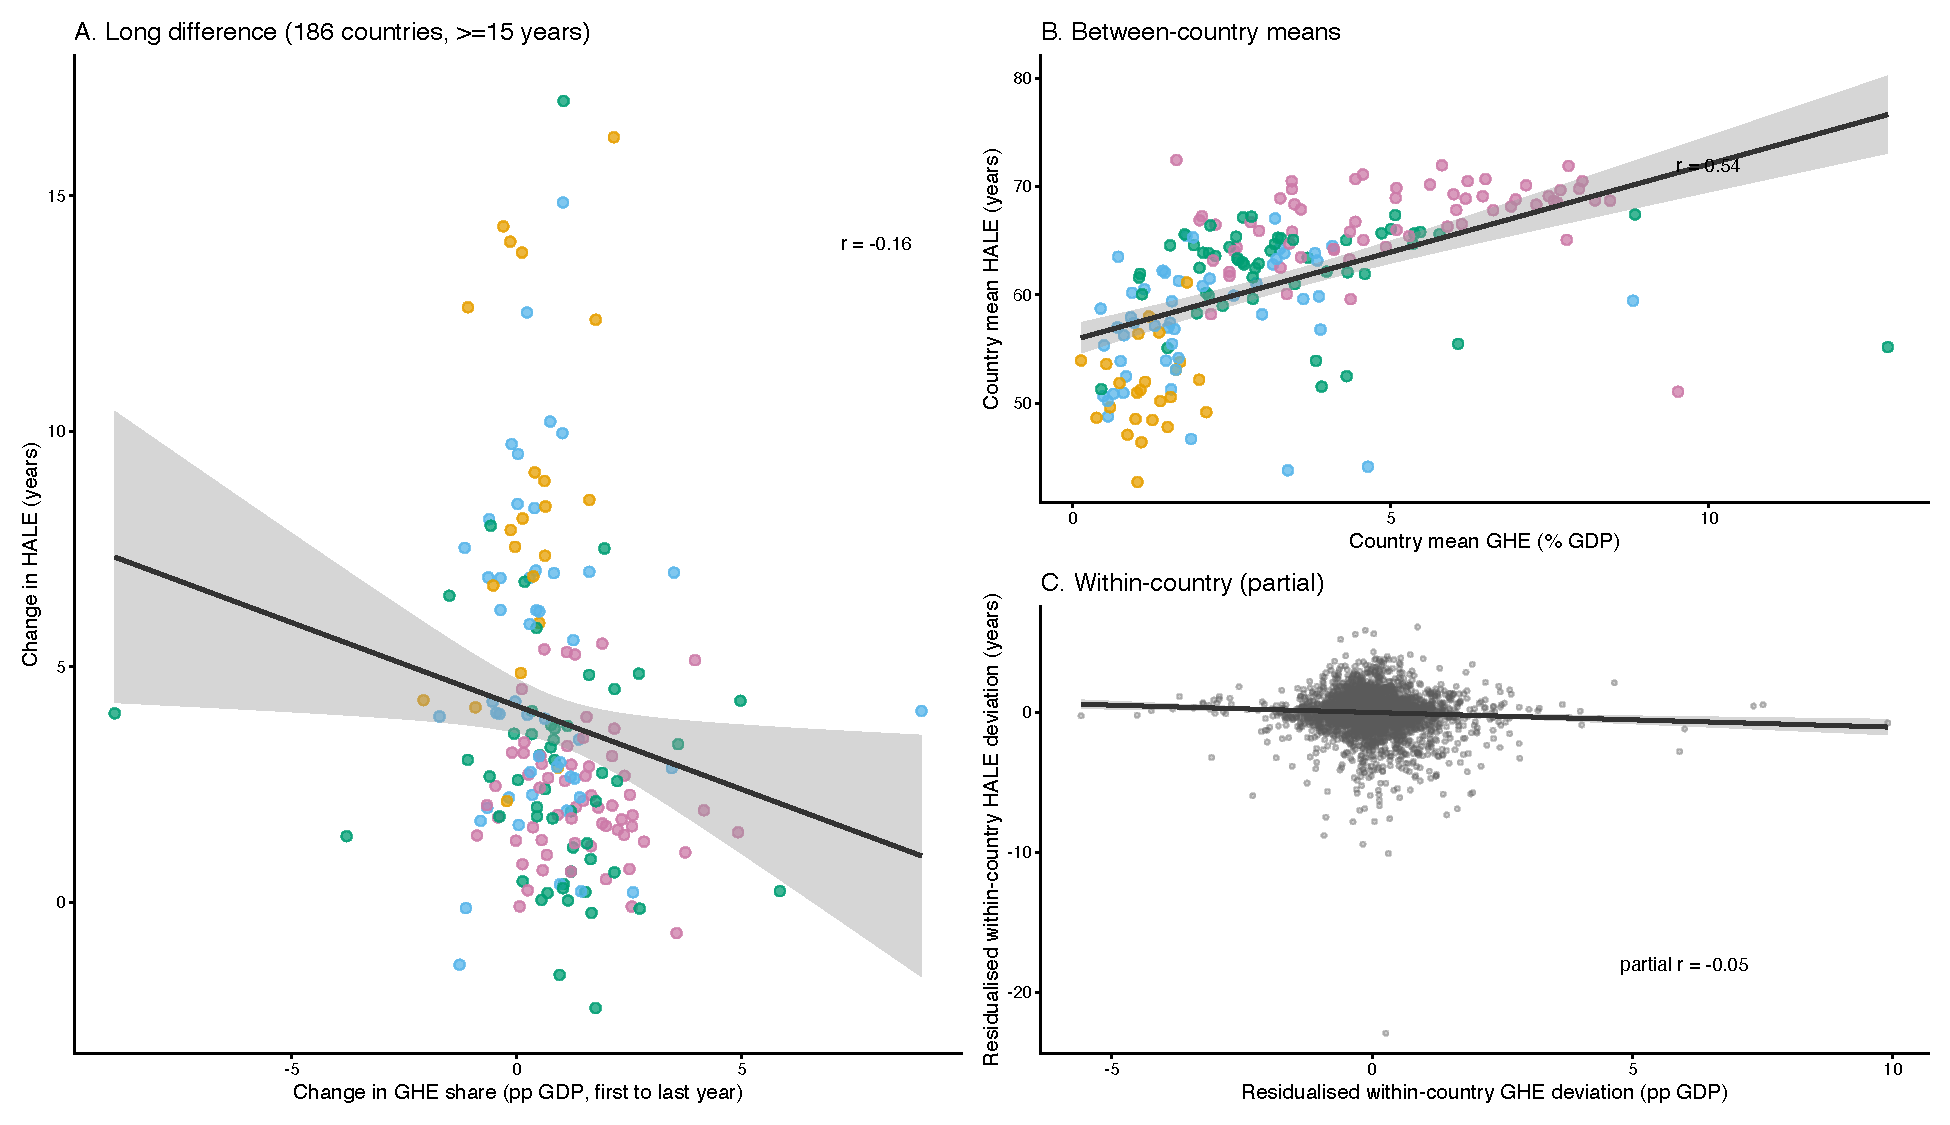
\includegraphics[width=\textwidth]{../results/figures/fig1_longdiff_bw.pdf}
\caption{\textbf{Between-country versus within-country variation in the GHE--HALE relationship.}
\textbf{A:} Long-difference analysis: change in HALE versus change in GHE share (earliest to latest available year) for 186 countries with $\geq$15 years of data; the association was small and negative ($r = -0{\textperiodcentered{}}16$; long-difference regression $-0{\textperiodcentered{}}33$, $p = 0{\textperiodcentered{}}034$), and 37 countries experienced HALE gains despite declining GHE shares. \textbf{B:} Country-level means show a strong positive correlation ($r = 0{\textperiodcentered{}}54$), reflecting the development gradient. \textbf{C:} Within-country deviations residualised on covariates show essentially no correlation (partial $r = -0{\textperiodcentered{}}05$). This decomposition illustrates why cross-sectional associations do not identify within-country effects. Point colours in A indicate income group.}
\label{fig:longdiff}
\end{figure}

\begin{figure}[H]\centering
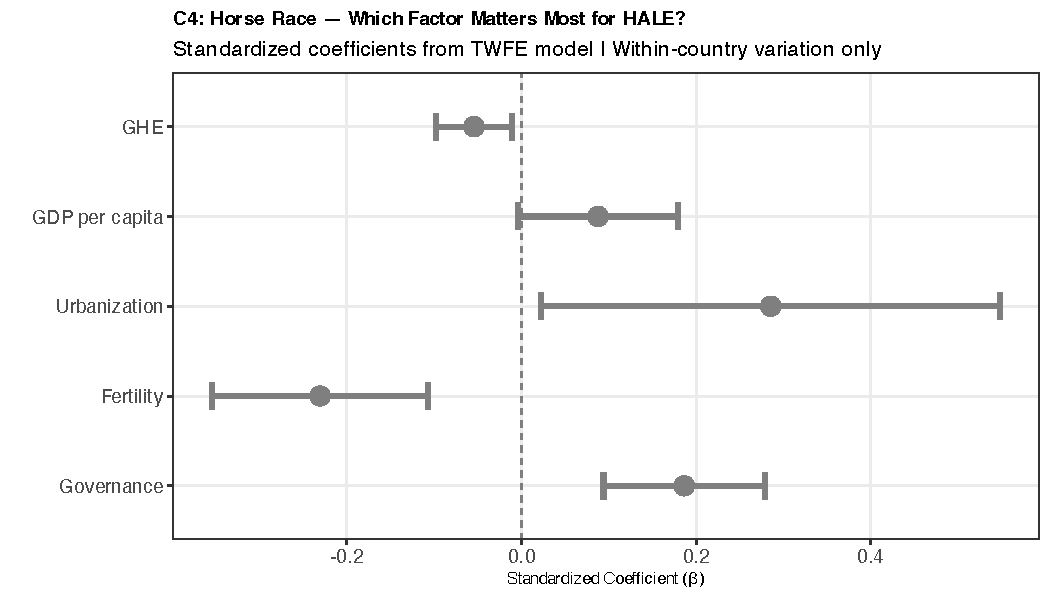
\includegraphics[width=0.90\textwidth]{../results/figures/C4_horse_race.pdf}
\caption{\textbf{Comparative standardised-coefficient model.} Standardised TWFE coefficients with 95\% CIs comparing the within-country associations of five major determinants with HALE, ordered by absolute magnitude. Urbanisation, fertility, log GDP per capita, and governance quality all show stronger associations than GHE. The unique within-$R^2$ contribution of GHE is 0{\textperiodcentered{}}004.}
\label{fig:horserace}
\end{figure}

\begin{figure}[H]
\centering
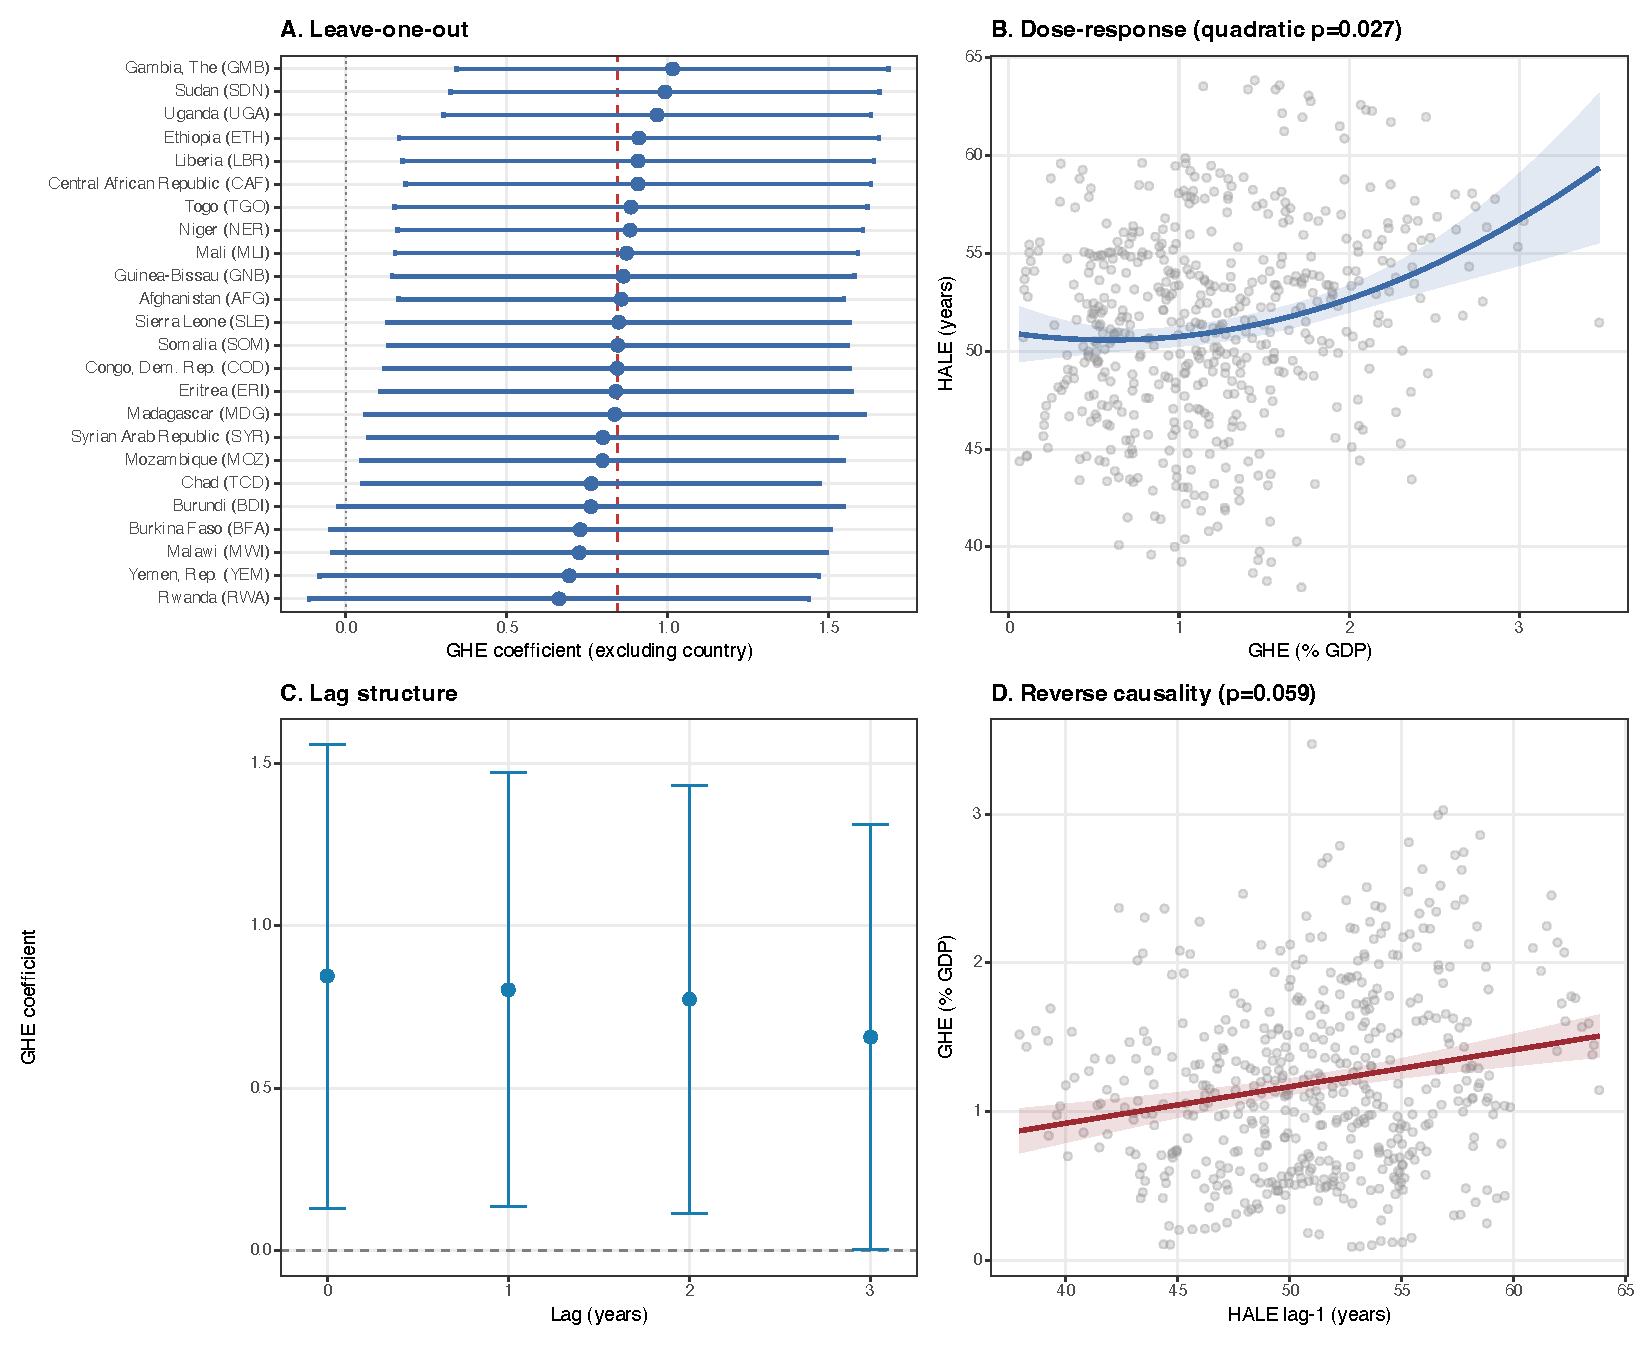
\includegraphics[width=\textwidth]{../results/figures/fig_lic_summary.pdf}
\caption{\textbf{Low-income country evidence: four converging analyses.}
\textbf{A:} Leave-one-out: all 23 re-estimated LIC coefficients remain
positive after iteratively excluding each country (range $+0{\textperiodcentered{}}663$ to
$+1{\textperiodcentered{}}016$). \textbf{B:} Dose-response: the quadratic term is positive and
significant ($+0{\textperiodcentered{}}52$, $p = 0{\textperiodcentered{}}027$), indicating a convex shape with
larger marginal associations at higher GHE; this is driven by few high-GHE
observations and weakens when Rwanda is excluded. \textbf{C:} Lag structure: association peaks at
contemporaneous $t$ and decays monotonically. \textbf{D:} Reverse causality: past HALE does not predict future GHE ($p > 0{\textperiodcentered{}}3$ for all lags); the contemporaneous association was borderline ($p = 0{\textperiodcentered{}}059$), compatible with coincident measurement rather than lagged reverse causation. Enlarged standalone versions of the four panels are provided in Supplementary Figures S9--S12.}
\label{fig:lic_summary}
\end{figure}



\end{document}
